\documentclass{article}
\usepackage{amsmath, amssymb, amssymb}
\usepackage{tikz}
\usetikzlibrary{3d}

\begin{document}
\begin{center}
    \begin{LARGE}
        \textbf{Introduction to Electromagnetism}
    \end{LARGE}
\end{center}

\section{Coulomb's Law}

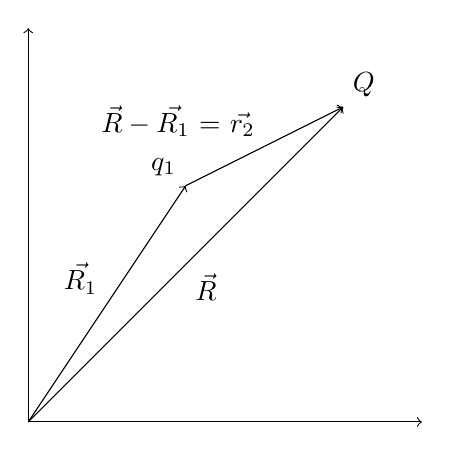
\begin{tikzpicture}
    \draw[->] [black] (0,0) -- (0, 5);
    \draw[->] [black] (0,0) -- (5, 0);
    \draw[black] (0,0) -- (2,2) node[anchor=north west] {$\vec{R}$};
    \draw[->] [black] (2,2) -- (4,4) node[anchor=south west] {$Q$};
    \draw[black] (0, 0) -- (1,1.5) node[anchor=south east] {$\vec{R_1}$};
    \draw[black, ->] (1,1.5) -- (2,3) node[anchor=south east] {$q_1$};
    \draw[black] (2,3) -- (3,3.5) node[anchor=south east] {$\vec{R} - \vec{R_1}$ = $\vec{r_2}$};
    \draw[->] [black] (3,3.5) -- (4,4);

\end{tikzpicture}
the force on $Q$ due to $q_1$ is given by:
\[\vec{F_1} = \frac{1}{4\pi\epsilon_0} \frac{q_1Q}{r_1^2} \hat{r_1}\]

If there was another charge $q_2$ at $\vec{r_2}$: 

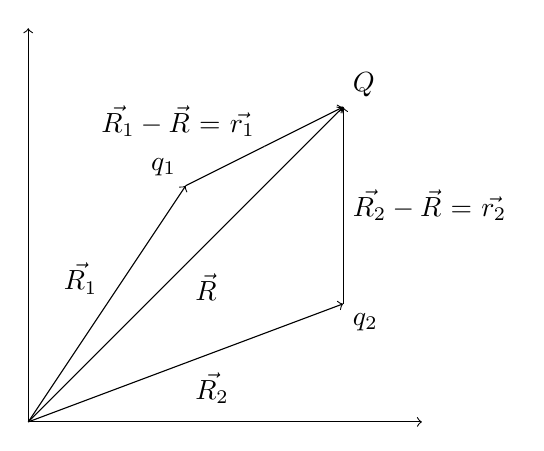
\begin{tikzpicture}
    \draw[->] [black] (0,0) -- (0, 5);
    \draw[->] [black] (0,0) -- (5, 0);
    \draw[black] (0,0) -- (2,2) node[anchor=north west] {$\vec{R}$};
    \draw[->] [black] (2,2) -- (4,4) node[anchor=south west] {$Q$};
    \draw[black] (0, 0) -- (1,1.5) node[anchor=south east] {$\vec{R_1}$};
    \draw[black, ->] (1,1.5) -- (2,3) node[anchor=south east] {$q_1$};
    \draw[black] (2,3) -- (3,3.5) node[anchor=south east] {$\vec{R_1} - \vec{R}$ = $\vec{r_1}$};
    \draw[->] [black] (3,3.5) -- (4,4);
    \draw[black] (0, 0) -- (2,0.75) node[anchor=north west] {$\vec{R_2}$};
    \draw[black, ->] (2,0.75) -- (4,1.5) node[anchor=north west] {$q_2$};
    \draw[black] (4,1.5) -- (4,2.75) node[anchor=west] {$\vec{R_2} - \vec{R}$ = $\vec{r_2}$};
    \draw[->] [black] (4,2.75) -- (4,4);

\end{tikzpicture}

The force on $Q$ due to $q_2$ is given by:
\[\vec{F_2} = \frac{1}{4\pi\epsilon_0} \frac{q_2Q}{r_2^2} \hat{r_2}\]

And the net charge on $Q$ is given by:
\[\vec{F} = \vec{F_1} + \vec{F_2}\]
\[\vec{F} = \frac{1}{4\pi\epsilon_0} \frac{q_1Q}{r_1^2} \hat{r_1} + \frac{1}{4\pi\epsilon_0} \frac{q_2Q}{r_2^2} \hat{r_2}\]

If there were $n$ charges, the net force on $Q$ would be:
\[\vec{F} = \sum_{i=1}^n \frac{1}{4\pi\epsilon_0} \frac{q_iQ}{r_i^2} \hat{r_i}\]
\[\vec{F} = Q \sum_{i=1}^n \frac{1}{4\pi\epsilon_0} \frac{q_i}{r_i^2} \hat{r_i}\]

where $\sum_{i=1}^n \frac{1}{4\pi\epsilon_0} \frac{q_i}{r_i^2} \hat{r_i}$ is the electric field $\vec{E}$ at $\vec{R}$ due to the $n$ charges.

\paragraph{Field}
A value, vector or tensor, that is defined for every point in space and time. \\[1pt] 

\section{Vector Calculus}

\paragraph{Vectors} 
A vector is a quantity that is said to transform like a displacement. \\[1pt]

\subsection{Operations on Vectors}
\begin{itemize}
    \item \textbf{Addition}: $\vec{A} + \vec{B} = \vec{C}$
    
        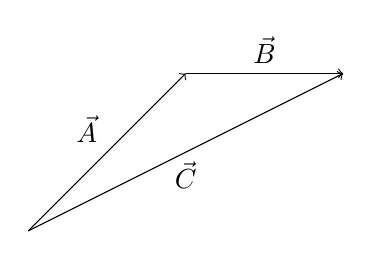
\begin{tikzpicture}
            \draw[black] (0,0) -- (1,1) node[anchor=south east] {$\vec{A}$};
            \draw[black, ->] (1,1) -- (2,2);
            \draw[black] (2,2) -- (3,2) node[anchor=south] {$\vec{B}$};
            \draw[black, ->] (3,2) -- (4,2);
            \draw[black] (0,0) -- (2,1) node[at end, anchor=north ] {$\vec{C}$};
            \draw[black, ->] (2,1) -- (4,2);
        \end{tikzpicture}

    \item \textbf{Subtraction:} $\vec{A} - \vec{B} = \vec{C}$
    
        \begin{tikzpicture}
            \draw[black] (0,0) -- (1,1) node[anchor=south east] {$\vec{C}$};
            \draw[black, ->] (1,1) -- (2,2);
            \draw[black, ->] (4,2) -- (6,2) node[anchor=south] {$\vec{B}$};
            \draw[black, <-] (2,2) -- (3,2) node[anchor=south] {$\vec{-B}$};
            \draw[black] (3,2) -- (4,2);
            \draw[black] (0,0) -- (2,1) node[at end, anchor=north ] {$\vec{A}$};
            \draw[black, ->] (2,1) -- (4,2);
        \end{tikzpicture}

    \item \textbf{Multiplication by a scalar: } $c\vec{A} = \vec{C}$
    \item \textbf{Dot Product: } $\vec{A}.\vec{B} = AB\cos(\theta)$.
        Dot product is a scalar. It is commutative and distributive.
    \item \textbf{Cross Product: } $\vec{A} \times \vec{B} = AB\sin(\theta) \hat{n}$
        where $\hat{n}$ is the unit vector perpendicular to the plane containing $\vec{A}$ and $\vec{B}$.
    \end{itemize}

        Cross product is a vector. It is anti-commutative and distributive.
    \subsection{Component form of a Vector: }
    A vector $\vec{A}$ can be written as:
    \[\vec{A} = A_x \hat{i} + A_y \hat{j} + A_z \hat{k}\]
    where $\hat{i}, \hat{j}, \hat{k}$ are unit vectors along the $x, y, z$ axes respectively.

    Given that $\vec{A} = A_x \hat{i} + A_y \hat{j} + A_z \hat{k}$ and $\vec{B} = B_x \hat{i} + B_y \hat{j} + B_z \hat{k}$, we can perform the following operations:
    \begin{itemize}
        \item \textbf{Addition (and Subtraction):} $\vec{A} + \vec{B} = (A_x + B_x) \hat{i} + (A_y + B_y) \hat{j} + (A_z + B_z) \hat{k}$
        \item \textbf{Multiplication by a scalar: } $c\vec{A} = cA_x \hat{i} + cA_y \hat{j} + cA_z \hat{k}$, where $c$ is a scalar.
        \item \textbf{Dot Product: } $\vec{A}.\vec{B} = A_xB_x + A_yB_y + A_zB_z$
        \item \textbf{Modulus: } $|\vec{A}| = \sqrt{A_x^2 + A_y^2 + A_z^2}$
        \item \textbf{Cross Product: } $\vec{A} \times \vec{B} = (A_yB_z - A_zB_y) \hat{i} + (A_zB_x - A_xB_z) \hat{j} + (A_xB_y - A_yB_x) \hat{k}$
            This can also be written in a determinant form:
            \[\vec{A} \times \vec{B} = \begin{vmatrix}
                \hat{i} & \hat{j} & \hat{k} \\
                A_x & A_y & A_z \\
                B_x & B_y & B_z
            \end{vmatrix}\]
    \end{itemize}
    \subsection{Triple Product: }
    \paragraph*{Scalar Triple Product: } $\vec{A}.(\vec{B} \times \vec{C}) = \vec{B}.(\vec{C} \times \vec{A}) = \vec{C}.(\vec{A} \times \vec{B})$
    Geometrically the scalar triple product is the volume of the parallelepiped formed by the three vectors.
    \paragraph*{Vector Triple Product: } $\vec{A} \times (\vec{B} \times \vec{C}) = \vec{B}(\vec{A}.\vec{C}) - \vec{C}(\vec{A}.\vec{B})$

\section{Differential Calculus}
\subsection{'Ordinary' Derivative: } $\frac{df}{dx} = \lim_{h \to 0} \frac{f(x+h) - f(x)}{h}$
Geometrically, the derivative is the slope of the tangent to the curve at a point.

\subsection{Gradient:} Consider a scalar, T, which exists at every point in space. 
\[d T = \left(\frac{\partial T}{\partial x}\right)dx + \left(\frac{\partial T}{\partial y}\right)dy + \left(\frac{\partial T}{\partial z}\right)dz\]
This can the written in the dot product form as:
\[d T = \left(\frac{\partial T}{\partial x}\hat{x} + \frac{\partial T}{\partial y}\hat{y} + \frac{\partial T}{\partial z}\hat{z} \right) \cdot (dx \hat{x} + dy \hat{y} + dz \hat{z} )\]
this is denoted as:
\[d T = \nabla T \cdot d\vec{r}\]
Here, we treat $\nabla$ as an operator. It takes a scalar and returns a vector.

\paragraph*{The $\nabla$ operator: } \[\nabla = \hat{x} \frac{\partial}{\partial x} + \hat{y} \frac{\partial}{\partial y} + \hat{z} \frac{\partial}{\partial z}\]

\subsection{Divergence: } Consider a vector, $\vec{A}$, which exists at every point in space. The divergence of $\vec{A}$ is defined as:
\[ \nabla \cdot \vec{A} = \left(\hat{x} \frac{\partial}{\partial x} + \hat{y} \frac{\partial}{\partial y} + \hat{z} \frac{\partial}{\partial z}{}\right) \cdot \left(A_x \hat{x} + A_y \hat{y} + A_z \hat{z}\right)\]
\[ \nabla \cdot \vec{A} = \frac{\partial A_x}{\partial x} + \frac{\partial A_y}{\partial y} + \frac{\partial A_z}{\partial z}\]

It behaves like a dot product, and is a scalar.

\subsection{Curl: } Consider a vector, $\vec{A}$, which exists at every point in space. The curl of $\vec{A}$ is defined as:
\[\nabla \times \vec{A}  = \begin{vmatrix}
    \hat{x} & \hat{y} & \hat{z} \\
    \partial/\partial x & \partial/\partial y & \partial/\partial z \\    
    A_x & A_y & A_z 
\end{vmatrix}\]

It behaves like a cross product, and is a vector.

\subsection{Second Derivatives: }
\begin{itemize}
    \item \textbf{Divergence of a Gradient: } $\nabla \cdot \left(\nabla T\right)$
    \[ \nabla \cdot \left(\nabla T\right)  = \left(\hat{x} \frac{\partial}{\partial x} + \hat{y} \frac{\partial}{\partial y} + \hat{z} \frac{\partial}{\partial z}\right) \cdot \left(\frac{\partial T}{\partial x} \hat{x} + \frac{\partial T}{\partial y} \hat{y} + \frac{\partial T}{\partial z} \hat{z}\right)\]
    \[ \nabla \cdot \left(\nabla T\right)  = \left(\frac{\partial^2 T}{\partial x^2} + \frac{\partial^2 T}{\partial y^2} + \frac{\partial^2 T}{\partial z^2}\right)\]
    It is denoted by $\nabla^2 T$ and is called the Laplacian of $T$.
    \paragraph*{Note:} Laplacian of a vector is theoretically not defined. But when $\nabla^2 \vec{A}$ is written, it means:
    \[\nabla^2 \vec{A} = \left(\nabla^2 A_x\right) \hat{x} + \left(\nabla^2 A_y\right) \hat{y} + \left(\nabla^2 A_z\right) \hat{z}\]
    \item \textbf{Curl of a Gradient: } $\nabla \times \left(\nabla T\right)$ 
    \[\nabla \times \left(\nabla T\right) = 0\]
    Curl of a gradient is always zero.
    \item \textbf{Gradient of Divergence: } $\nabla \left(\nabla \cdot \vec{A}\right)$
    \item \textbf{Divergence of Curl: } $\nabla \cdot \left(\nabla \times \vec{A}\right)$
    \[\nabla \cdot \left(\nabla \times \vec{A}\right) = 0\]
    Divergence of a Curl is always zero.
    \item \textbf{Curl of Curl: } $\nabla \times \left(\nabla \times \vec{A}\right)$
    \[\nabla \times \left(\nabla \times \vec{A}\right) = \nabla \left(\nabla \cdot \vec{A}\right) - \nabla^2 \vec{A}\]
\end{itemize}

\section{Integral Calculus}

\subsection{Line Integral: }
Consider a vector field $\vec{V}$ and a curve $C$ joining points $a$ and $b$. The line integral of $\vec{V}$ along $C$ is defined as:
\[\int_{aP}^{b} \vec{V} \cdot d\vec{l}\]
where $d\vec{l}$ is the differential displacement along the curve $C$.

when $C$ is a closed figure, it is written as:
\[\oint \vec{V} \cdot d\vec{l}\]
\subsection{Surface Integral: }
Consider a vector field $\vec{V}$ and a surface $S$. The surface integral of $\vec{V}$ over $S$ is defined as:
\[\int_{S} \vec{V}\cdot \vec{da}\]
where $\vec{da}$ is the differential area vector of the surface $S$.

When $S$ is a closed surface:
\[\oint \vec{V}\cdot\vec{da}\]

\subsection{Volume Integral: }
Consider a scalar field $T$ and a volume $V$. The volume integral of $T$ over $V$ is defined as:
\[\int_{V} T dV\]
\\
If we consider a vector field $\vec{A}$, then:
\[\int \vec{A} dV\]
\[\hat{x} \int A_x dV + \hat{y} \int A_y dV + \hat{z} \int A_z dV\]

In Cartesian coordinates:
\[dV = dx dy dz\]

In Spherical Polar coordinates:
\[dV = r^2 \sin(\theta) dr d\theta d\phi\]

\subsection{Fundamental Theorem of Calculus: }
If $f(x)$ is a continuous function and $F(x)$ is the anti-derivative of $f(x)$, then:
\[\int_{a}^{b} f(x) = F(b) - F(a)\]
\\

\begin{itemize}
    \item \textbf{Fundamental Theorem for Gradients: }

Consider a scalar field $T$ and a curve $C$, from $\vec{a}$ to $\vec{b}$, then:
\[\int_{\vec{a}}^{\vec{b}} \nabla T \cdot d\vec{l} = T(\vec{b}) - T(\vec{a})\]
If the curve is a closed curve, then:
\[\int_{\vec{a}}^{\vec{b}} \nabla T \cdot d\vec{l} = 0\]

\item \textbf{Fundamental Theorem for Divergence: } a.k.a Gauss' Theorem, Green's Theorem or divergence theorem.
Consider a vector field $\vec{A}$ and a volume $V$, then:
\[\int_{V}\left(\vec{\nabla} \cdot \vec{v}\right) = \oint \vec{v}.\vec{ds}\]
where $ds$  is the differential area vector of the surface $S$.

\item \textbf{Fundamental Theorem for Curl: } a.k.a Stokes' Theorem.
Consider a vector field $\vec{A}$ and a surface $S$, then:
\[\int_{S}\left(\vec{\nabla} \times \vec{v}\right) \vec{da}= \oint \vec{v}.\vec{dl}\]
where $dl$  is the differential displacement vector along the boundary curve $C$ of the surface $S$.

\end{itemize}

\section{Dirac Delta Function: }
\subsection{One-Dimensional Dirac Delta Function: }
It is a function that is zero everywhere except at $x = 0$ and has an integral of 1. It is defined as:
\[\delta(x) = \begin{cases}
    \infty & x = 0 \\
    0 & x \neq 0
\end{cases}\]
and
\[\int_{-\infty}^{\infty} \delta(x) dx = 1\]
Mathematically, it is not a function, i.e., don't tell your maths profs that its a function.

\subsection{Three-Dimensional Dirac Delta Function: }
It is a function that is zero everywhere except at $\vec{r} = \vec{r_0}$ and has a volume integral of 1. It is defined as:

\[\delta^3(\vec{r}) = \begin{cases}
    \infty & (x,y,z) = (0,0,0) \\
    0 & \text{everywhere else}
\end{cases}\]
\[\delta^3(\vec{r}) = \delta(x)\delta(y)\delta(z)\]
and
\[\int_{\text{all space}} \delta^3\left(\vec{r}\right) d\tau = \int_{-\infty}^{\infty}\int_{-\infty}^{\infty}\int_{-\infty}^{\infty}\delta(x)\delta(y)\delta(z) dx dy dz\]

Generalizing the function:
\[\int_{\text{all space}} f(r)\delta^3\left(r-a\right) d\tau = f(a)\]

\section{Electrostatics}
\subsection{Electric Field}
\begin{center}
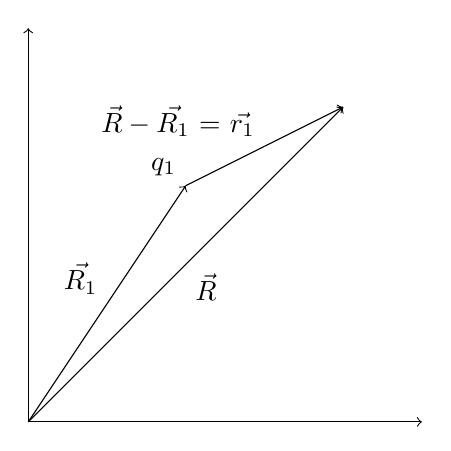
\begin{tikzpicture}
    \draw[->] [black] (0,0) -- (0, 5);
    \draw[->] [black] (0,0) -- (5, 0);
    \draw[black] (0,0) -- (2,2) node[anchor=north west] {$\vec{R}$};
    \draw[->] [black] (2,2) -- (4,4);
    \draw[black] (0, 0) -- (1,1.5) node[anchor=south east] {$\vec{R_1}$};
    \draw[black, ->] (1,1.5) -- (2,3) node[anchor=south east] {$q_1$};
    \draw[black] (2,3) -- (3,3.5) node[anchor=south east] {$\vec{R} - \vec{R_1}$ = $\vec{r_1}$};
    \draw[->] [black] (3,3.5) -- (4,4);
\end{tikzpicture}
\end{center}
The Electric Field at $\vec{R}$ due to $q_1$ is given by:
\[\vec{E} = \frac{1}{4\pi\epsilon_0} \frac{q_1}{r_1^2} \hat{r_1}\]

If there is another charge present:
\begin{center}
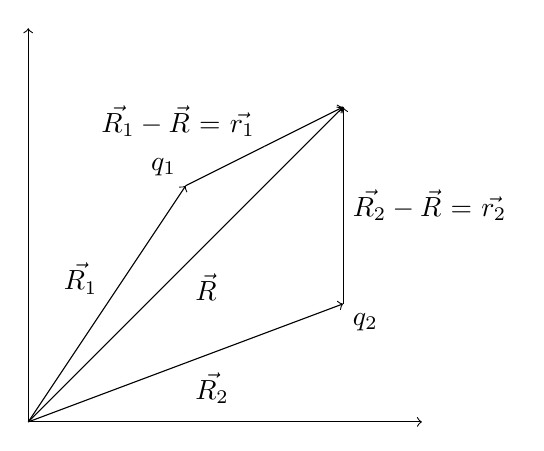
\begin{tikzpicture}
    \draw[->] [black] (0,0) -- (0, 5);
    \draw[->] [black] (0,0) -- (5, 0);
    \draw[black] (0,0) -- (2,2) node[anchor=north west] {$\vec{R}$};
    \draw[->] [black] (2,2) -- (4,4);
    \draw[black] (0, 0) -- (1,1.5) node[anchor=south east] {$\vec{R_1}$};
    \draw[black, ->] (1,1.5) -- (2,3) node[anchor=south east] {$q_1$};
    \draw[black] (2,3) -- (3,3.5) node[anchor=south east] {$\vec{R_1} - \vec{R}$ = $\vec{r_1}$};
    \draw[->] [black] (3,3.5) -- (4,4);
    \draw[black] (0, 0) -- (2,0.75) node[anchor=north west] {$\vec{R_2}$};
    \draw[black, ->] (2,0.75) -- (4,1.5) node[anchor=north west] {$q_2$};
    \draw[black] (4,1.5) -- (4,2.75) node[anchor=west] {$\vec{R_2} - \vec{R}$ = $\vec{r_2}$};
    \draw[->] [black] (4,2.75) -- (4,4);

\end{tikzpicture}
\end{center}
\[\vec{E} = \frac{1}{4\pi\epsilon_0} \left(\frac{q_1}{r_1^2}\hat{r_1} + \frac{q_2}{r_1^2}\hat{r_2}\right)\]

\subsubsection*{Principle of Superposition:}
The net electric field at $\vec{R}$ due to $n$ charges is given by:

\[E = \frac{1}{4\pi\epsilon_0} \left( \sum_{i = 1}^{n} \frac{q_i}{r_i^2}\hat{r_i} \right)\]

\subsubsection*{Question:}
\begin{tikzpicture}
    \draw[<->, black] (-2.5,0) -- (2.5,0);
    \draw[->, black] (0,0) -- (0, 4);
    \draw[->, black] (0,0) -- (0, 3);
    \draw[-, black] (0,0) -- (0, 1.5) node[anchor=south west] {$\vec{z}$};
    \draw[-, black] (0,0) -- (1,0) node[anchor=north] {$d/2$};
    \draw[-, black] (0,0) -- (-1,0) node[anchor=north] {$d/2$};
    \draw[->, black] (1, 0) -- (2, 0) node[anchor=south west] {$q$};
    \draw[->, black] (-1, 0) -- (-2, 0) node[anchor=south east] {$q$};
    \draw[-, black] (2, 0) -- (1, 1.5) node[anchor=south west] {$\vec{r_1}$};
    \draw[-, black] (-2, 0) -- (-1, 1.5) node[anchor=south east] {$\vec{r_2}$};
    \draw[->, black] (1, 1.5) -- (0, 3);
    \draw[->, black] (-1, 1.5) -- (0, 3);

\end{tikzpicture}

Consider two charges, $q$, placed at $r = \pm \frac{d}{2}$ respectively. Find the electric field at $z$.

\subsubsection*{Answer}
\[\vec{E} = \frac{1}{4\pi\epsilon_0} \left( \frac{q}{\left(\frac{d}{2}\right)^2 + z^2} \hat{r_1} + \frac{q}{\left(\frac{d}{2}\right)^2 + + z^2} \hat{r_2} \right)\]
\[\vec{E} = \frac{1}{4\pi\epsilon_0} \left( \frac{2q}{z^2 + \frac{d^2}{4}}\right) \left(\frac{z}{\sqrt{z^2 + \frac{d^2}{4}}}\hat{z}\right)\]
\[\vec{E} = \frac{1}{4\pi\epsilon_0} \left( \frac{2qz}{\left(z^2 + \frac{d^2}{4}\right)^{\frac{3}{2}}}\right) \hat{z}\]
\\
Now, if $z$ is very large (but not infinity):

\[\vec{E} = \frac{1}{4\pi\epsilon_0} \left( \frac{2q}{z^2}\right)\left(1 + \frac{d^2}{4z^2}\right)^{\frac{-3}{2}} \hat{z}\]
this can be approximated to:
\[\vec{E} = \frac{1}{4\pi\epsilon_0} \left( \frac{2q}{z^2}\right)\left(1 - \frac{3d^2}{8z^2}\right) \hat{z}\]

Similar methods can be used to find the electric field for any discrete charge distribution.

\subsection{Continuous Charge Distribution}
\subsubsection{Linear Charge Distribution}
Consider a linear Charge distribution, $\lambda$ of length $l$, along the $x$ axis. The electric field at point $P$ is given by: \\
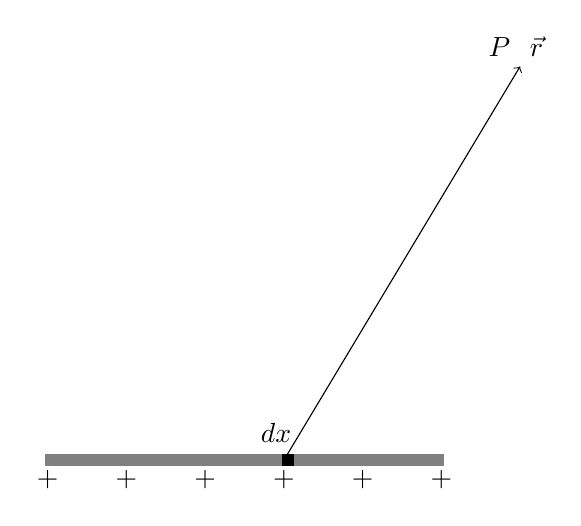
\begin{tikzpicture}
    \filldraw[ultra thick, gray] (0,-.05) rectangle (5,0.05);
    \filldraw[ultra thick, black] (3,-.05) rectangle (3.1,0.05);
    \node[anchor=south] at (2.9, 0.1) {$dx$};
    \draw[->] [black] (3,0) -- (6, 5) node[anchor=south west] {$\vec{r}$};
    \node[anchor=north] at (0,0) {+};
    \node[anchor=north] at (1,0) {+};
    \node[anchor=north] at (2,0) {+};
    \node[anchor=north] at (3,0) {+};
    \node[anchor=north] at (4,0) {+};
    \node[anchor=north] at (5,0) {+};
    \node[anchor=south east] at (6,5) {$P$};
\end{tikzpicture}\\
The Electric Field at point $P$ due to $dx$ is given by:
\[d\vec{E} = \frac{1}{4\pi \epsilon_0} \frac{\lambda dx}{r^2} \hat{r}  \]
Hence, the electric field at point $P$ due to the entire linear charge distribution is given by:
\[\vec{E} = \int_{\text{length $l$}} \frac{1}{4\pi \epsilon_0} \frac{\lambda dx}{r^2} \hat{r} \]

\subsubsection{Surface Charge Distribution}
Consider a surface charge distribution, $\sigma$ of area $A$, on the $xy$ plane. The electric field at point $P$ is given by:\\
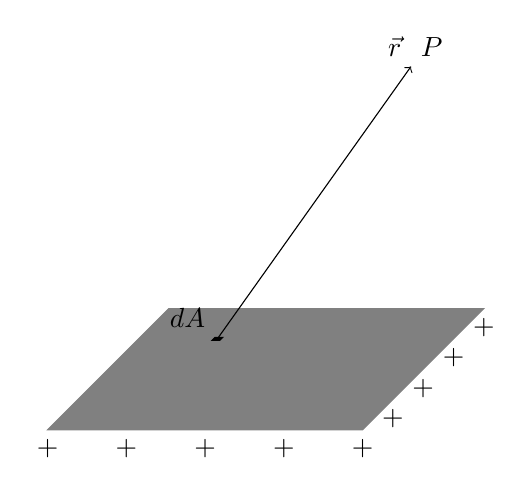
\begin{tikzpicture}
    \filldraw[gray] (-2,0,-2) -- (2,0,-2) -- (2,0,2) -- (-2,0,2) -- cycle;
    \filldraw[black] (-1.05,0,-1.05) -- (-0.95,0,-1.05) -- (-0.95,0,-0.95) -- (-1.05,0,-0.95) -- cycle node[anchor=south east] {$dA$};
    \draw[black, ->](-1, 0, -1) -- (3,5,3) node[anchor=south east] {$\vec{r}$};
    \node[anchor=north] at (2,0,2) {+};
    \node[anchor=north] at (1,0,2) {+};
    \node[anchor=north] at (0,0,2) {+};
    \node[anchor=north] at (-1,0,2) {+};
    \node[anchor=north] at (-2,0,2) {+};
    \node[anchor=north] at (2,0,-2) {+};
    \node[anchor=north] at (2,0,-1) {+};
    \node[anchor=north] at (2,0,0) {+};
    \node[anchor=north] at (2,0,1) {+};
    \node[anchor=south west] at (3,5,3) {$P$};
\end{tikzpicture}\\
The Electric Field at point $P$ due to $dA$ is given by:
\[ d\vec{E} = \frac{1}{4 \pi \epsilon} \frac{\sigma dA}{r^2} \hat{r} \]
Hence, the electric field at point $P$ due to the entire surface charge distribution is given by:
\[ \vec{E} = \int_{\text{area $A$}} \frac{1}{4 \pi \epsilon} \frac{\sigma dA}{r^2} \hat{r} \]

\subsubsection{Volume Charge Distribution}
Consider a volume charge distribution, $\rho$ of volume $V$, in space. The electric field at point $P$ is given by:\\
%make a potato and find the electric field at the centre

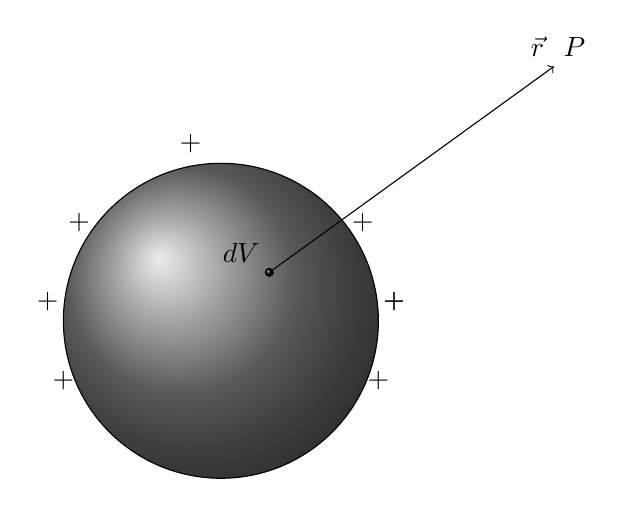
\begin{tikzpicture}
    \filldraw[ball color=gray] (0,0,0) circle (2);
    \filldraw[ball color=black] (1,1,1) circle (0.05) node[anchor=south east] {$dV$};
    \draw[->, black] (1,1,1) -- (5,4,2) node[anchor=south east] {$\vec{r}$};
    \node[anchor=south west] at (5,4,2) {$P$};
    \node[anchor=south] at (2.2,0,0) {+};
    \node[anchor=south] at (1.8,1,0) {+};
    \node[anchor=south] at (2,-1,0) {+};
    \node[anchor=south] at (-2.2,0,0) {+};
    \node[anchor=south] at (-1.8,1,0) {+};
    \node[anchor=south] at (0,2.4,1) {+};
    \node[anchor=south] at (2.2,0,0) {+};
    \node[anchor=south] at (-2,-1,0) {+};
    

\end{tikzpicture}\\
The electric field at point $P$ due to $dV$ is given by:
\[ d\vec{E} = \frac{1}{4 \pi\epsilon_0} \frac{\rho dV}{r^2} \hat{r} \]
Hence, the electric field at point $P$ due to the entire volume charge distribution is given by:
\[ \vec{E} = \int_{\text{volume }V} \frac{1}{4 \pi \epsilon} \frac{\rho dV}{r^2} \hat{r} \]


\section{Divergence and Curl of Electric Field}
\subsection{Flux and Gauss' Law}
\paragraph{Flux}
The Electric Flux through a surface $S$ is defined as:
\[\Phi_E = \int_{S} \vec{E} \cdot \vec{da}\]

Now, if the surface $S$ is a closed surface, then:
\[\Phi_E = \oint \vec{E} \cdot \vec{da}\]

\paragraph*{A charge in a sphere}

\paragraph*{A charge in a cube}


\paragraph{Gauss' Law}
As seen with the above two examples of the electric flux through a closed surface, the electric flux through a closed surface is proportional to the charge enclosed by the surface. This is known as Gauss' Law. Mathematically, it is written as:
\[\oint \vec{E} \cdot \vec{da} = \frac{Q_{enc}}{\epsilon_0}\]
where $Q_{enc}$ is the charge enclosed by the surface.
This is also know as the integral form of Gauss' Law or the integral form of Maxwell's first equation.

To write it in the form of a differential equation:\\
\[Q_{enc} = \int_{V}\rho d\tau \]
\[\int_V (\vec{\nabla} \cdot \vec{E}) dV = \oint \vec{E} \cdot \vec{da} \]
\[ \int_V (\vec{\nabla} \cdot \vec{E}) dV = \int_{V}\rho d\tau \]
As this is true for all volumes, we can write:
\[\vec{\nabla} \cdot \vec{E} = \frac{\rho}{\epsilon_0}\]
This is the differential form of Gauss' Law or Maxwell's first equation.

\subsubsection{Divergence of Electric Field}

The Electric Field at a point $\vec{r}$ due to a continuous charge distribution at $\vec{r'}$ is given by:

\[\vec{E}(\vec{r}) = \frac{1}{4 \pi \epsilon_0} \int_{\text{all space}} \frac{\hat{\gamma}}{\gamma^2} \rho(\vec{r'}) d\tau' \]
taking the divergence of the above function
\[ \vec{\nabla} \cdot \vec{E}(\vec{r}) = \frac{1}{4 \pi \epsilon_0} \int_{\text{all space}} \vec{\nabla} \cdot \left(\frac{\hat{\gamma}}{\gamma^2}\right) \rho(\vec{r'}) d\tau' \]
\[\vec{\nabla}\cdot\frac{\hat{\gamma}}{\gamma^2} = 4 \pi \delta^3(\gamma)\]
\[ \vec{\nabla} \cdot \vec{E} = \frac{1}{4 \pi \epsilon_0} \int 4 \pi \delta^3(r-r') \rho(r') d\tau' = \frac{1}{\epsilon_0} \rho(r)\]

\subsubsection{Application of Gauss' Law} 

\begin{itemize}

\item \textbf{Spherical Charge Distribution}
Consider a spherical charge distribution of radius $\gamma$ and net charge $Q$. The electric field at a point $r$ is given by:\\

\item \textbf{Infinitely Long Linear Charge Distribution}

\item \textbf{Infinitely Large Surface Charge Distribution}

\end{itemize}

\end{document} 